Ebben a fejezetben kerülnek azok az adatok bemutatásra, amelyek alapján az első lépésben a modell
paraméterei meghatározásra kerülnek, illetve ha kész a modell ezen adatsorok új elemeivel
lehetséges megelőlegezett, de egyben még is megalapozott jóslatot tenni arra, hogy épp mekkora az
ország bruttó nemzeti összterméke.

Mivel a gazdaság az egyik legbonyolultabb rendszer a világon, így végtelen sok paraméteres
modelleket lehetne felállítani, amely a működését próbálja valamilyen formában megfogni. Ráadásul a
különböző szereplők, mint az utóbbi évtizedekben látjuk, sokszor irracionálisan viselkednek,
döntéseik sokszor kontextus függők, így egy teljes modellt felépíteni egy szakdolgozat keretében
lehetetlen vállalkozás.

A következő lehetőség, amely ebben a dolgozatban kihasználásra kerül, olyan fontos gazdasági
jellemzők összegyűjtése, amelyek bizonyítottan jól jósolják be a gazdaság egyes szektorainak vagy
egészének teljesítményét.

A projektfeladat keretében a következő jellemzőket választottam:

\begin{itemize}
    \item Energia:
          \begin{itemize}
              \item Üzemanyag fogyasztás (benzin és diesel)
              \item Üzemanyag árak (benzin és diesel)
              \item Gázárak
              \item Elektromos árak
          \end{itemize}
    \item Időjárás:
          \begin{itemize}
              \item Hőmérséklet
              \item Csapadék
              \item Levegő szennyezettség
          \end{itemize}
    \item Budapesti Értéktőzsde
    \item Gazdasági adatok
          \begin{itemize}
              \item Infláció
              \item Munkaerőpiac
          \end{itemize}
\end{itemize}

\section{Üzemanyag fogyasztás}

A mobilitás alapja még mindig a robbanómotoros közlekedési eszközök, így azok ára nagyon fontos
indikátora a gazdasági aktivitásnak. Minél alacsonyabb az ára az üzemanyagnak, annál több ember
teheti meg, hogy autózzon és annál több vállalkozásnak éri meg a termékeit szállítmányozni. És
természetesen minél alacsonyabb az üzemanyag ára, annál többet fogyasztanak belőle.

A magyarországi üzemanyag fogyasztást a Százhalombattán finomított üzemanyagok biztosítják messze a
legnagyobb százalékban. Százhalombattán továbbra is Barátság vezetéken szállított orosz uráli
típusú nyersolajat finomítanak még mindig, bár lassan folynak az átalakítási folyamatok, hogy más
forrásból tudjon fogadni nyers termékeket. Bár mindig megfigyelhető volt némi árkülönbség a brent
és az uráli típusú termékek között, az orosz-ukrán háború kiszélesedése után bevezetett szankciók
miatt a kereslet lecsökkent az uráli nyersolajra és így az ára nyomottá vált.

Ennek ellenére nincs különösebb kiskereskedelmi árkülönbség azon szomszédos országokkal összevetve,
ahol nem orosz termékeket dolgoznak fel. Így a nyereség legnagyobb részben a MOL-nál csapódik le.
Így elég, sőt indokolt a hazai árakkal dolgozni.

\begin{figure}[htbp]
    \centering
    \includegraphics[width=1\textwidth, height=0.8\textheight, keepaspectratio]{../figures/petrol_consumption.png}
    \caption{A magyar GDP alakulása szektorok szerint}\label{fig:petrol_consumption}
\end{figure}

Az ábrán zölddel a dízel, kékkel a benzin fogyasztás látható. Sötétebbel a projektfeladat keretében
vizsgált időszak (2015--2019) adatai lettek szedve. Megfigyelhetjük, a 2008-as válság miatti
fogyasztás visszaesés. Az erőteljes gazdasági növekedés 2014 körül tért vissza, utána viszont
meredeken emelkedett a fogyasztás. Olyan beruházások megvalósítása, mint a debreceni BMW gyár
építését megelőző tereprendezése, hónapokra 10--15\%-kal is meg tudták a dízel fogyasztást növelni.

A Covid lezárások visszavetették mindkét üzemanyag típus fogyasztását, de a benzin fogyasztásában
arányaiban jobban visszaesett, mert a benzint személygépkocsik használják nagyobb arányban és a
magánszemélyek mozgása sokáig korlátozva volt.

Ezzel szemben a 2022-ben bevezetett 480 forintos benzinársapka újból magasba emelte a fogyasztást,
sőt akkortájt még a benzinturizmus is megjelent a határaink mentén.

\section{Üzemanyag árak}

Az üzemanyag árak rugalmasabban alakulnak az üzemanyag fogyasztásánál, hiszen például megkezdett
beruházásokat nem hagynak félben amiatt, ha véletlenül kicsit drágább lesz a dízel.

Az előbb láthattuk tehát, hogy az üzemanyag kereslet rövidtávon rugalmatlan, addig a kínálatot
legalább két tényező befolyásolja még:
\begin{itemize}
    \item A különböző nemzetközi kartellszervezetek döntései.
    \item A piac várakozása, hiszen ha növekedés a konszenzusos várakozás, akkor megéri többet termelni,
          hiszen úgy is meg fogják venni. Így viszont túlkínálat is kialakulhat.
\end{itemize}

Épp utóbbira lehet példa a 2015--18-as időszak. A 2022-es választásra való felkészülést kísérő
kiköltekezés gyorsan megemelte az inflációt, majd az Ukrájnában kiújuló ellenségeskedés miatti aggodalom,
majd 2022 végén életbe lépő szankciók miatti csökkenő kereslet egekbe emelte az üzemanyag árakat. Ennek tartott ellent néhány hónapig a benzinársapka.

\begin{figure}[htbp]
    \centering
    \includegraphics[width=1\textwidth, height=0.8\textheight, keepaspectratio]{../figures/petrol_prices.png}
    \caption{A magyar GDP alakulása szektorok szerint}\label{fig:petrol_prices}
\end{figure}

\section{Jegybanki alapkamat}

A Magyar Nemzeti Bank törvényben előírt, de a közvélemény által is ismert feladata kettős, ugyanis
a jegybank felelős azért, hogy az inflációt a 2--4\%\-os tartományban tartsa. (A másik feladata, ha
teljesülni látszik az első, akkor a gazdasági növekedés támogatása.) Ehhez a legerősebb eszköze ---
nagyon leegyszerűsítve a folyamatot --- a jegybanki alapkamat. A kétszintű bankrendszer, amilyen a
magyar bankrendszer is, úgy működik, hogy a jegybank hitelt nyújt a professzionális pénzügyi
szervezeteknek az alapkamatnak megfelelő kamattal. A kereskedelmi bankok pedig a saját működési
költségüket és a profitjukat ráteszik az alapkamatra és ezen feltételek mellett kínálják
termékeiket a piacon.

Értelemszerűen, ha a jegyban magasabb alapkamatot tart fenn, akkor a kereskedelmi bankok is még
magasabb hitelkamatokkal működnek. Ami viszont azt jelenti, hogy mind a lakosságnak mind vállalati
szektornak megdrágul a finanszírozás. Az emelkedő kamatokkal jellemezhető hiteleket egyre kevesebben
vállalják be, törlik az újabb projekteket vagy csak elhalasztják őket, így végül csökken a
pénzmennyiség gazdaságban. Ez pedig az alapkamat emelésének célja, mert egyre lassabban emelkednek a
termékek árai, egyes esetekben akár csökkenhet is. Ez pedig definíció szerint az infláció
megszűnése. Hogy körbeérjen a folyamat, ekkor a nemzeti bankok elkezdhetik csökkenteni az
alapkamatot, ami ellentétes folyamatok indít el, nevezetesen több pénzt juttat a gazdaságba,
amit növekedést indukál. Ez pedig a magyar jegybank másodlagos feladata.

Magyarországon a rendszerváltás utáni időszakot, illetve a Covid válság utáni időszakot nagyon
magas inflációs környezet jellemezte. Természetesen a MNB élt a kamatemelés eszközével és
visszaszorította az inflációt alacsonyabb szintre. De ez költségvetési megszorításokkal is járt
valamilyen formában, bár nem minden esetben nevezte a gazdaságirányítás megszorításnak őket.
Illetve az előbb említett intézkedések a gazdasági növekedést is lassították.

Ezért megkerülhetetlenül fontos változó a GDP adat becslésében.

Megyjegyzendő, hogy a jegybanki alapkamat a kamatdöntő ülések során kerül meghatározásra és sokszor
a döntés a nem változtatás. Így ez a változót, a legtöbb változó esetével ellentétben, nem kell
interpolálni azokra a napokra, amikor nem volt kamatdöntő ülés, hanem elég őket az utolsó döntés
szinjén tartani.

\section{Teljes villamosenergia-felhasználás Magyarországon}

A magyar teljes bruttó villamosenergia-felhasználás a vizsgált 2015--2019-es időszakban nagyjából
100 és 140 GWh között ingadozott, ahogyan azt a lentebbi ábrán is látszik. Ebben fogyasztási
adatsorban természetesen nemcsak a lakossági, de a vállalati szektor energiafogyasztása is benne
van.

\begin{figure}[htbp]
    \centering
    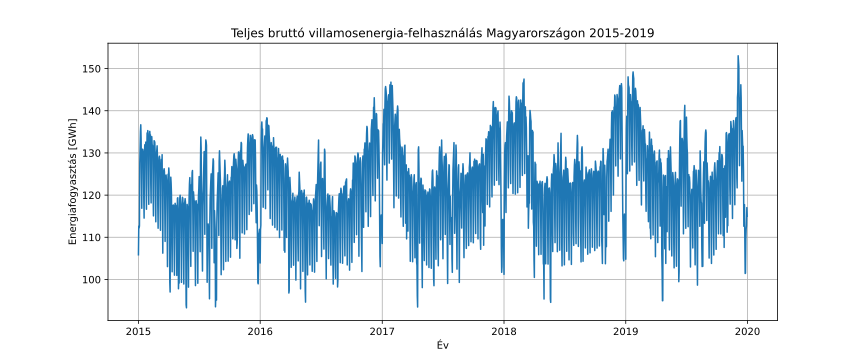
\includegraphics[width=1\textwidth, height=0.8\textheight, keepaspectratio]{../figures/mavir.png}
    \caption{Teljes bruttó villamosenergia-felhasználás Magyarországon}\label{fig:mavir}
\end{figure}

Az éves szezonalitás azonnal szembetűnő. A heti periódusokat viszont szabad szemmel nem lehet az
ábrán megfigyelni, de a korábbi frekvencianalízisre alapuló esettanulmány erős jelenlétet mutatott
ki. Az ábrán megfigyelhetők továbbá a téli és a nyári fogyasztási csúcsok, illetve az év végi
leállások is. És végül egy kis trendszerűséget is észre lehet venni, hiszen 2015 zömében 130 GWh
alatti mért értékeket hozott, addig 2017-től egyre gyakoribbak a 140 GWh feletti értékek is illetve
az átlag is, mintha tolódna felfelé.

Mivel mind a szezonalitás mind a trendszerűség megfigyelhető, vizsgálódásunk tárgya a SARIMA modell
felépítése lesz.

A megközelítésünk lényege az, hogy felosztjuk a 2015--2019 időszakot egy négy és egy egyéves
időszakra. Az első időszak adatai szolgálnak a modell betanítására, míg az utolsó 20\% pedig az
eredmények verifikálására. Egészen pontosan 2019.\ január 1.--jére helyezzük magunkat és
feltételezzük, hogy már rendelkezésünkre áll a betanított modell. A modell segítségével
előrejelezzük az aznapi fogyasztási adatot, majd éjfélkor, a tényadat birtokában, újrakalibráljuk a
modell, hogy január másodikán is a legpontosabb becslést tudjuk tenni. És ezt a
becslési--újrakalibrálási ciklust ismételjük meg az egész 2019--es év folyamán.

\subsection{Adatok dekomponálása}

Ebben a lépésben az a célunk, hogy a rendelkezésünkre álló adatok alapján, a feltételezéseinknek
megfelelően az adatokat három komponensre bontsuk fel:

\begin{itemize}
    \item trendszerűen emelkedő/csökkenő részre
    \item szezonalitáson alapuló részre és
    \item a maradványra
\end{itemize}

A helyzetet, ebben az esetben az is bonyolítja, hogy nem is egy, hanem legalább két ciklikusság is
kimutatható az adatokból (heti és évi ciklusok).

Első lépésben azonban azonosítsuk be a trendszerű részt:

\begin{equation}
    y_{trend}(t) = \frac{1}{N} \sum_{i=t-\frac{N-1}{2}}^{t+\frac{N-1}{2}} y_i
\end{equation}

Láthatjuk, hogy a trendszerű részt egy $N$--elemű csúszóablakkal számíthatjuk ki. Ez az ablak az
$y$ $t$-t megelőző $\frac{N}{2}$ tagjától a $t$--t követő $+\frac{N}{2}$ tagot átlagolja.

Így a visszamaradó tagot, a trendszerű résztől megtisztított részt a következőképpen kapjuk:

\begin{equation}
    y_{detrended}(t) = y_t - y_{trend}(t) = y_t - \frac{1}{N} \sum_{i=t-\frac{N-1}{2}}^{t+\frac{N-1}{2}} y_i
\end{equation}

A fenti módszerrel előállított trendszerű komponenst láthatjuk a következő ábrán:

\begin{figure}[htbp]
    \centering
    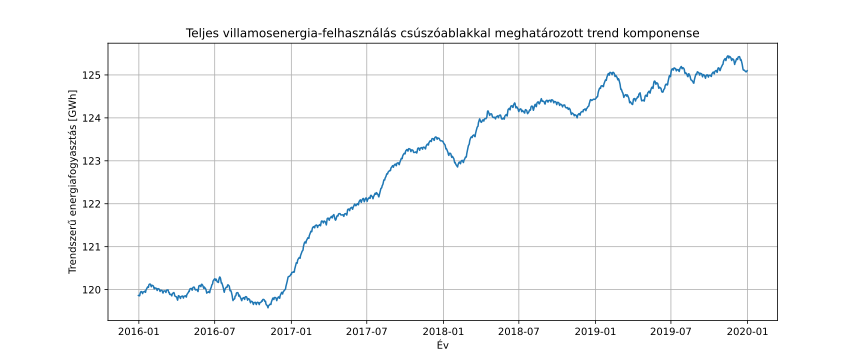
\includegraphics[width=1\textwidth, height=0.8\textheight, keepaspectratio]{../figures/mavir_trend_by_hand.png}
    \caption{Villamosenergia-felhasználás csúszóablakkal meghatározott trend komponense}\label{fig:mavir_trend_by_hand}
\end{figure}

A második lépés a ciklikus tagok azonosítása és dekomponálása. Ha a modell feltevésünk teljesen
helyes, akkor az ezutáni lépésből visszamaradó értékek már a fehér zajt jelentik.

A frekvenciák felkutatására a már korábban megismert ACF-t (autokorrelációs függvény) és PACF
(parciális autokorrelációs függvényt) használjuk.

\begin{figure}[htbp]
    \centering
    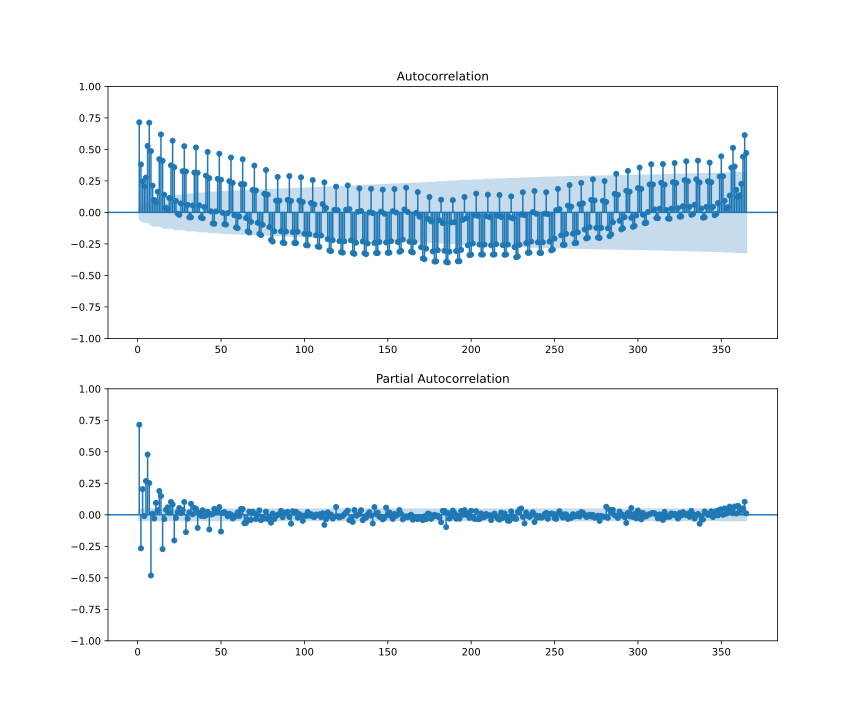
\includegraphics[width=1\textwidth, height=0.8\textheight, keepaspectratio]{../figures/mavir_residual_acf_by_hand.png}
    \caption{A trend komponenstől megtisztított adat autokorrelációs függvényei}\label{fig:mavir_residual_acf_by_hand}
\end{figure}

A fenti ábrákon láthatjuk, hogy valóban a heti frekvencia milyen magas értéket kapott, de
megfigyelhető az éves frekvecia is. Sőt a hét napnak egész többszörösei is magas értékeket kaptak
az autokorrelációs függvényektől, ami előrevetíti, hogy nem lesz tökéletes az illeszkedés, azaz
nemcsak fehérzak marad vissza.

\subsection{MLTS}

A fentebbi algoritmust az idők során tovább fejlesztették, hiszen több kihívással is szembe kell
nézni, ha azt használja az ember:

\begin{itemize}
    \item ha N=365 napos ciklust feltételezünk, akkor az adatsor elején és végén is elvesztük fél évnyi
          adatot
    \item ha az adatsorban vannak kiugróbb adatok, akkor a trendnek azonosított értékben is lesz ugrás
\end{itemize}

Az Multi-Seasonal Time Series Loess-t (MLTS) ilyen helyzetekre hozták létre, így

\begin{itemize}
    \item nincs adatvesztés
    \item a trendvonalat a Locally Estimated Scatterplot Smoothing (LOESS) algoritmus kisimítja
    \item ráadásul, miután a szezonalitásokat azonosította és dekomponálta, visszatér a trend értékekre is és
          pontosítja őket
\end{itemize}

\begin{figure}[htbp]
    \centering
    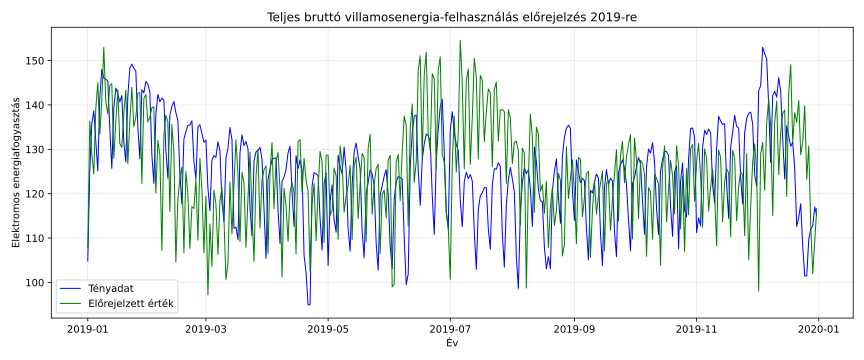
\includegraphics[width=1\textwidth, height=0.8\textheight, keepaspectratio]{../figures/mavir_daily_forecast.png}
    \caption{Teljes bruttó villamosenergia-felhasználás Magyarországon}\label{fig:mavir_daily_forecast}
\end{figure}

Természetesen

\section{Budapesti Értéktőzsde}

\begin{figure}[htbp]
    \centering
    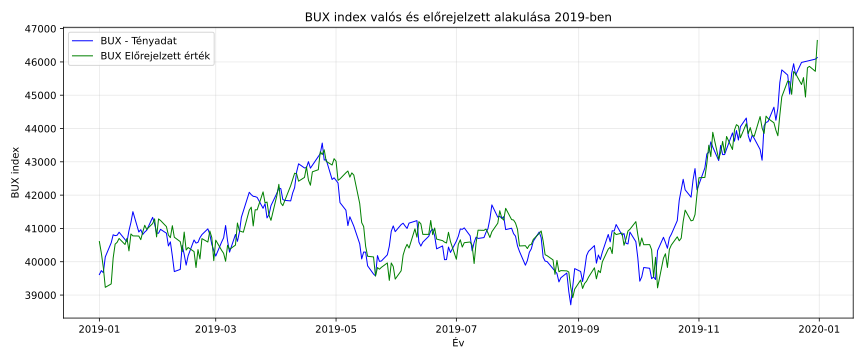
\includegraphics[width=1\textwidth, height=0.8\textheight, keepaspectratio]{../figures/bux_daily_forecast.png}
    \caption{Teljes bruttó villamosenergia-felhasználás Magyarországon}\label{fig:bux_daily_forecast}
\end{figure}